% !TeX encoding = windows-1251
\documentclass[12pt,a4paper]{article}
\usepackage[mag=1000]{newlistok}
\usepackage{tikz}\usetikzlibrary{calc, patterns}

\УвеличитьШирину{.3cm}
\УвеличитьВысоту{2.2cm}
% \renewcommand{\spacer}{\vspace{2pt}}



\begin{document}



\Заголовок{Принцип Дирихле}
\НадНомеромЛистка{179 школа, 7Б.}
\НомерЛистка{2}
\ДатаЛистка{09.2017}
\СоздатьЗаголовок

\задача  В коробке 50 конфет трёх видов. Докажите, что конфет какого-то вида не менее 17.
\кзадача


\задача Какое наименьшее количество учеников должно быть в школе, чтобы гарантированно можно было найти трёх учеников, отмечающих день рождения в один день?
\кзадача

\задача Докажите, что существуют две различные степени семёрки, оканчивающиеся на одну и ту же комбинацию из трёх цифр. %такие, что три их последние цифры совпадают.
\кзадача

\задача В соревнованиях по бегу участвуют 100 спортсменов. Известно, что среди любых 12 из них найдутся двое знакомых между собой. Докажите, что как бы ни раздали спортсменам стартовые номера (не обязательно от 1 до 100), найдутся два знакомых спортсмена, номера которых начинаются с одной и той же цифры.
\кзадача

\ввзадача
\пункт[Принцип Дирихле] Докажите, что если в $n$ клетках сидит не менее
$n+1$ кроликов, то найдётся клетка, в которой сидит не менее двух кроликов.\\
\пункт[Обобщённый принцип Дирихле] Докажите, что если в $n$ клетках сидит не менее
$k$ кроликов, то найдётся клетка, в которой сидит не менее $k/n$ кроликов. Как следует
понимать это утверждение, если $k$ не делится на $n$ нацело?\\
\пункт Что в предыдущих задачах <<клетки>>, а что --- <<кролики>>?
\кзадача

\задача Докажите, что если в $n$ клетках сидит менее
$\frac{n(n-1)}{2}$ кроликов, то найдутся две клетки, в которых сидит одинаковое количество кроликов (может быть, ни одного)
\кзадача

\задача Для награждения по итогам школьного конкурса имеется 70 конфет. При каком наибольшем количестве конкурсантов им можно будет раздать конфеты так, что все они получат разное и не меньшее 3 количество конфет?
\кзадача

\задача На заводе 7 цехов, в которых работает 360 человек. Докажите, что в каких-то пяти из этих цехов работает не менее 258 человек.
\кзадача

\задача Пять мальчиков собрали 53 гриба, причём известно, что никакие двое не собрали грибов поровну. Докажите, что какие-то трое из них собрали не менее 36 грибов.
\кзадача

\задача В коробке 70 карандашей. Докажите, что найдутся либо 9 карандашей одного цвета, либо 9 карандашей разного цвета.
\кзадача

\задача В кинотеатре 7 рядов по 10 мест каждый. Группа из 50 детей сходила на утренний сеанс, а потом на вечерний. Докажите, что найдутся двое детей, которые на утреннем сеансе сидели в одном ряду и на вечернем тоже сидели в одном ряду.
\кзадача

\задача Числа от 1 до 9 некоторым образом разбиты на три группы. Докажите, что произведение чисел в одной из групп не меньше 72.
\кзадача

\задача Можно ли 100 гирь массами $1,2,3,\ldots,99,100$ разложить на 10 кучек разной массы так, чтобы выполнялось условие: чем тяжелее кучка, тем меньше в ней гирь?
\кзадача

\задача У 10 девочек было по 10 конфет. Каждая девочка подарила несколько конфет другим (конфеты, полученные в подарок, девочки оставляют себе). В результате у всех девочек оказалось разное число конфет. Докажите, что какая-то из девочек подарила конфет не меньше, чем у неё их оказалось в конце.
\кзадача

\сзадача На складе имеется несколько ящиков общей массой 10 тонн, причём масса каждого не превосходит тонны. Какое наименьшее количество трёхтонок нужно заказать, чтобы точно суметь вывезти их все за один раз?
\кзадача


	\ЛичныйКондуит{0mm}{6mm}
\vfill
\begin{center}
\large Смотри примеры решений на обороте
\end{center}
\newpage

\раздел{Примеры задач с решениями}
\пример
В классе 30 учеников. Докажите, что найдутся трое учеников, родившихся в одном и том же месяце.
\кпример
\решение Предположим противное: пусть в каждом месяце родилось меньше трёх
учеников, то есть не более двух. Тогда всего учеников не более $2 \cdot 12 = 24$ человек.  Значит, наше предположение неверно, и найдётся месяц, в котором родилось не менее трёх учеников.
\крешение

\пример
Шесть мальчиков съели 13 конфет. Докажите, что найдутся два мальчика, которые съели конфет поровну (возможно, что ни одной).
\кпример
\решение Предположим, что все мальчики съели разное число конфет. Расположим их по возрастанию числа съеденных конфет. Тогда первый съел не меньше 0 конфет, второй съел больше первого, то есть не меньше~1, и т.д. Значит, всего они съели не меньше $0 + 1 + 2 + 3 + 4 + 5 = 15$ конфет, что противоречит условию. Значит наше предположение неверно, и найдутся два мальчика, съевшие одинаковое число конфет.
\крешение

\пример
В семи кабинетах стоят 107 парт. Докажите, что можно выбрать из этих кабинетов три, в которых вместе не меньше 47  парт.
\кпример
\решение Рассмотрим три кабинета, в которых находится больше всего парт. Предположим, что в них вместе не более 46 парт. Тогда в каком-то одном из них не более
15 парт (иначе всего в этих трёх кабинетах было бы не меньше $16 \cdot 3 = 48$ парт, что противоречит предположению.) Но тогда в оставшихся четырёх кабинетах не более $15 \cdot 4 = 60$ парт (поскольку выбрали три самых больших кабинета). А всего в семи кабинетах не более
46 + 60 = 106 парт, что противоречит условию. Значит предположение неверно, и найдутся три кабинета, в которых вместе не менее 47 парт.
\крешение

\пример
В походе участвовало 18 школьников. Докажите, что среди них либо были пять школьников из одного класса, либо в походе приняли участие школьники не
менее чем из пяти классов.\nobreak
\кпример
\решение Предположим, что в походе приняли участие школьники не более чем
четырёх классов, причем из каждого не более четырёх учащихся. Тогда всего в походе участвовало не более $4 \cdot 4 = 16$ учащихся, что противоречит условию. Значит предположение неверно, и в походе приняли участие либо школьники не менее чем пяти классов, либо не менее пяти учащихся из одного класса.
\крешение

%\GenXMLW

\end{document}

\newpage

{\bf Старая версия}


{\footnotesize \textbf{Принцип Дирихле.} Пусть есть $n$ ящиков и $n+1$ кроликов. Если расселить кроликов по ящикам, то найдется хотя бы один ящик, в котором
 окажутся не менее $2$ кроликов.}

\задача В мешке имеется $32$ красных шара, $29$ зеленых шаров, $45$ синих, $17$ желтых и по $30$ белых, черных и
серых (всего $213$ шаров). Сколько шаров необходимо вынуть из мешка, чтобы среди них гарантированно
нашлось $9$ шаров одного цвета? \кзадача

\задача Комиссия из $60$ человек провела $40$ заседаний, причем на каждом заседании присутствовали ровно $10$
членов комиссии. Докажите, что найдутся два члена комиссии, по крайней мере дважды встречавшиеся
на заседаниях. \\
{\tt Есть два решения: одно использует комбинаторику (для расчёта количества пар), другое не использует.}
 \кзадача

\задача
В таблице $10 \times 10$ расставлены \пункт числа от 1 до 100; \пункт произвольные целые числа, причем любые два числа в соседних клетках отличаются не более, чем на $5$. Докажите, что среди этих чисел найдутся два равных.
{\tt Это, конечно скорее задача на принцип крайнего, чем на принцип Дирихле}
\кзадача

\задача На шахматной доске стоит 44 ферзя. Докажите, что каждый из них бьёт какого-нибудь другого ферзя.
\кзадача

\задача В клетках таблицы $4 \times 4$ расставлено $6$ звездочек. Докажите, что из таблицы можно вычеркнуть две строки и два столбца так, что в оставшейся таблице звездочек не будет.
\кзадача

\задача Клетки доски $8 \times 8$ раскрашены в разные цвета. Назовём клетку {\it счастливой}, если хотя бы две соседние с ней по стороне клетки покрашены в тот же цвет. При каком наибольшем количестве цветов можно раскрасить доску так, что все клетки будут счастливыми?
\кзадача

\сзадача Восемь школьников решали 8 задач. Оказалось, что каждую задачу решили 5 школьников.
Докажите, что найдутся такие два школьника, что каждую задачу решил хотя бы один из них.
{\tt Опять используется комбинаторика. }
\кзадача



% \GenXMLW

\end{document}





































\putthere{169mm}{-11mm}{%
    %
    % пирамидка
      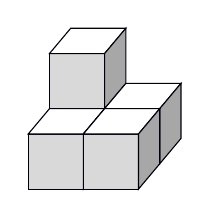
\begin{tikzpicture}
      [scale=.7
    % эти константы задают раскраску граней
      ,fil1/.style={draw=blue!5!black,fill=gray!00,thin}
      ,fil2/.style={draw=blue!5!black,fill=gray!30,thin}
      ,fil3/.style={draw=blue!5!black,fill=gray!69,thin}
      ]
    % эти константы задают наклон кубика
        \coordinate (d) at (50:.6);

        \coordinate (A) at (0,0);
        \coordinate (md) at ($ (0,0) - (d) $);
        \filldraw[fil2] (A) -- +(1,0) -- +(1,1) -- +(0,1) -- cycle;
        \filldraw[fil1] (A)++(1,1) -- ++(d) -- ++(-1,0) -- ++(md) -- cycle;
        \filldraw[fil3] (A)++(1,1) -- ++(d) -- ++(0,-1) -- ++(md) -- cycle;
        \coordinate (A) at ($(0,-1)+(md)$);
        \filldraw[fil2] (A) -- +(1,0) -- +(1,1) -- +(0,1) -- cycle;
        \filldraw[fil1] (A)++(1,1) -- ++(d) -- ++(-1,0) -- ++(md) -- cycle;
        \filldraw[fil3] (A)++(1,1) -- ++(d) -- ++(0,-1) -- ++(md) -- cycle;
        \coordinate (A) at (1,-1);
        \filldraw[fil2] (A) -- +(1,0) -- +(1,1) -- +(0,1) -- cycle;
        \filldraw[fil1] (A)++(1,1) -- ++(d) -- ++(-1,0) -- ++(md) -- cycle;
        \filldraw[fil3] (A)++(1,1) -- ++(d) -- ++(0,-1) -- ++(md) -- cycle;
        \coordinate (A) at ($(1,-1)+(md)$);
        \filldraw[fil2] (A) -- +(1,0) -- +(1,1) -- +(0,1) -- cycle;
        \filldraw[fil1] (A)++(1,1) -- ++(d) -- ++(-1,0) -- ++(md) -- cycle;
        \filldraw[fil3] (A)++(1,1) -- ++(d) -- ++(0,-1) -- ++(md) -- cycle;
       \end{tikzpicture}
}{5cm}{\risn Пирамида для $1^2+2^2$}
\vspace{-4mm}
\УстановитьГраницы{0truecm}{4truecm}


\сзадача Число $k^2$ можно представлять себе как объём параллелепипеда
$1\times k\times k$, а~сумму $1^2+2^2+\ldots+n^2$ --- как объём пирамиды,
сложенной из таких параллелепипедов. Будем обозначать эту пирамиду $Sq(n)$
(на рисунке 3 изображена пирамида $Sq(2)$ объёмом $1^2+2^2$).
Сложите из шести пирамид $Sq(n)$ параллелепипед.
Каковы его размеры и объём? Выведите
формулу для суммы $1^2+2^2+\ldots+n^2$.
\кзадача




\putthere{165mm}{-17mm}{%
    %
    % пирамидки
      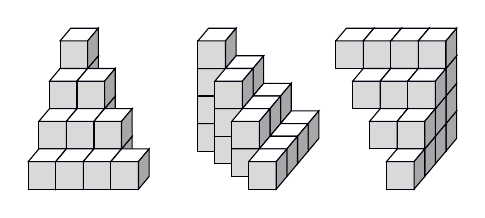
\begin{tikzpicture}
      [scale=.35
      ,fil1/.style={draw=blue!5!black,fill=gray!00,thin}
      ,fil2/.style={draw=blue!5!black,fill=gray!30,thin}
      ,fil3/.style={draw=blue!5!black,fill=gray!69,thin}
      ]
        \coordinate (d) at (50:.6);
        \coordinate (A1) at (0,0);
        \coordinate (A2) at (5,0);
        \coordinate (A3) at (10,0);
        \coordinate (md) at ($ (0,0) - (d) $);

        \foreach \x/\y/\z in {1/4/3, 1/4/4, 2/3/2, 1/3/3, 2/3/3, 3/2/1, 1/2/2, 2/2/2, 3/2/2, 1/1/1, 2/1/1, 3/1/1, 4/1/1}
        {
            \coordinate (A) at ($ (A1) + \x*(1,0) + \z*(0,1) + \y*(d)$);
            \filldraw[fil2] (A) -- +(1,0) -- +(1,1) -- +(0,1) -- cycle;
            \filldraw[fil1] (A)++(1,1) -- ++(d) -- ++(-1,0) -- ++(md) -- cycle;
            \filldraw[fil3] (A)++(1,1) -- ++(d) -- ++(0,-1) -- ++(md) -- cycle;
        }

        \foreach \x/\y/\z in {1/4/1, 1/4/2, 1/4/3, 1/4/4, 2/4/3, 2/3/1, 2/3/2, 2/3/3,   3/4/2, 3/3/2, 3/2/1, 3/2/2,  4/4/1, 4/3/1, 4/2/1, 4/1/1}
        {
            \coordinate (A) at ($ (A2) + \x*(1,0) + \z*(0,1) + \y*(d)$);
            \filldraw[fil2] (A) -- +(1,0) -- +(1,1) -- +(0,1) -- cycle;
            \filldraw[fil1] (A)++(1,1) -- ++(d) -- ++(-1,0) -- ++(md) -- cycle;
            \filldraw[fil3] (A)++(1,1) -- ++(d) -- ++(0,-1) -- ++(md) -- cycle;
        }

        \foreach \x/\y/\z in {4/4/1, 4/3/1, 4/2/1, 4/1/1, 1/4/4, 4/4/2, 4/3/2, 4/2/2, 2/4/4, 3/4/4, 4/4/3, 4/4/4,  2/3/3, 3/3/3, 4/3/3, 3/2/2, 4/2/2}
        {
            \coordinate (A) at ($ (A3) + \x*(1,0) + \z*(0,1) + \y*(d)$);
            \filldraw[fil2] (A) -- +(1,0) -- +(1,1) -- +(0,1) -- cycle;
            \filldraw[fil1] (A)++(1,1) -- ++(d) -- ++(-1,0) -- ++(md) -- cycle;
            \filldraw[fil3] (A)++(1,1) -- ++(d) -- ++(0,-1) -- ++(md) -- cycle;
        }

       \end{tikzpicture}
}{5cm}{\risn Интересные пирамиды}
\vspace{-4mm}
\УстановитьГраницы{0truecm}{6.4truecm}


\задача
\putthere{160mm}{-70mm}{%
    %
    % Таблица
    %
      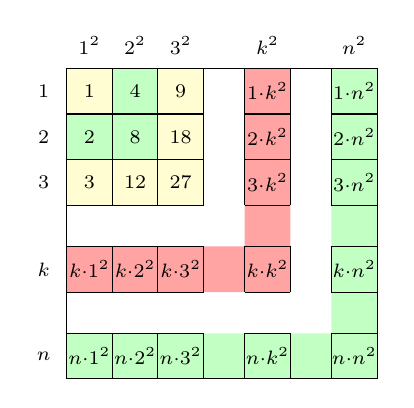
\begin{tikzpicture}
      [scale=.58
      ,fil1/.style={color=green!40!white,opacity=.6}
      ,fil2/.style={color=red!60!white,opacity=.6}
      ,fil3/.style={color=yellow!30!white,opacity=.6}
      ,lin/.style={color=black!100}
      ]
        \fill[fil1] (6.3,-0.5) -- (7.3,-0.5) -- (7.3, -7.3) -- (0.5,-7.3) -- (0.5,-6.3) -- (6.3,-6.3) -- cycle;
        \fill[fil2] (4.4,-0.5) -- (5.4,-0.5) -- (5.4, -5.4) -- (0.5,-5.4) -- (0.5,-4.4) -- (4.4,-4.4) -- cycle;
        \fill[fil3] (2.5,-0.5) -- (3.5,-0.5) -- (3.5, -3.5) -- (0.5,-3.5) -- (0.5,-2.5) -- (2.5,-2.5) -- cycle;
        \fill[fil1] (1.5,-0.5) -- (2.5,-0.5) -- (2.5, -2.5) -- (0.5,-2.5) -- (0.5,-1.5) -- (1.5,-1.5) -- cycle;
        \fill[fil3] (0.5,-0.5) -- (1.5,-0.5) -- (1.5, -1.5) -- (0.5,-1.5) -- cycle;
        \foreach \i in {1.5, 2.5, 3.5, 4.4, 5.4,  6.3}{
          \draw[lin] (0.5, -\i) -- (3.5, -\i);
          \draw[lin] (4.4, -\i) -- (5.4, -\i);
          \draw[lin] (6.3, -\i) -- (7.3, -\i);
          \draw[lin] (\i, -0.5) -- (\i, -3.5);
          \draw[lin] (\i, -4.4) -- (\i, -5.4);
          \draw[lin] (\i, -6.3) -- (\i, -7.3);
        }
        \draw[lin] (0.5, -0.5) -- (0.5, -7.3);
        \draw[lin] (0.5, -0.5) -- (7.3, -0.5);
        \draw[lin] (7.3, -7.3) -- (0.5, -7.3);
        \draw[lin] (7.3, -7.3) -- (7.3, -0.5);
        \draw (1, -1) node {$\scriptstyle 1$};
        \draw (2, -1) node {$\scriptstyle 4$};
        \draw (3, -1) node {$\scriptstyle 9$};
        \draw (1, -2) node {$\scriptstyle 2$};
        \draw (2, -2) node {$\scriptstyle 8$};
        \draw (3, -2) node {$\scriptstyle 18$};
        \draw (1, -3) node {$\scriptstyle 3$};
        \draw (2, -3) node {$\scriptstyle 12$};
        \draw (3, -3) node {$\scriptstyle 27$};
        \foreach \i in {1,2,3}
        {
          \draw (\i, -4.9) node {$\scriptstyle k\cdot\i^2$};
          \draw (4.9, -\i) node {$\scriptstyle\i\cdot k^2$};
          \draw (\i, -6.8) node {$\scriptstyle n\cdot\i^2$};
          \draw (6.8, -\i) node {$\scriptstyle\i\cdot n^2$};
          \draw (\i, 0) node {$\scriptstyle \i^2$};
          \draw (0, -\i) node {$\scriptstyle \i$};
        }

        \draw (4.9, -4.9) node {$\scriptstyle k\cdot k^2$};
        \draw (6.8, -4.9) node {$\scriptstyle k\cdot n^2$};
        \draw (4.9, -6.8) node {$\scriptstyle n\cdot k^2$};
        \draw (6.8, -6.8) node {$\scriptstyle n\cdot n^2$};
        \draw (4.9, 0) node {$\scriptstyle k^2$};
        \draw (6.8, 0) node {$\scriptstyle n^2$};
        \draw (0, -4.9) node {$\scriptstyle k$};
        \draw (0, -6.8) node {$\scriptstyle n$};

      \end{tikzpicture}
}{7cm}{}%{\risn Таблица умножения\\чисел и их квадратов}
На рисунке справа изображены несколько пирамид высоты~4,
каждая из них состоит из $T_1+T_2+T_3+T_4$ кубиков.
\пункт Выберите одну из пирамид на рисунке и нарисуйте её горизонтальные слои:
нижний, второй снизу, \dots , верхний.
\пункт Нарисуйте передний, второй спереди, \dots ,
задний слои выбранной пирамиды;
\пункт Нарисуйте самый левый, второй слева, \dots, самый правый слои выбранной пирамиды.
\пункт Сложите из шести пирамид такого вида параллелепипед. Каковы его размеры?
\ВосстановитьГраницы
\noindent\hspace*{-3.5mm}\пункт Как сложить параллелепипед из шести пирамид аналогичного вида,
но высоты $n$? Найдите формулу для суммы треугольных чисел $T_1+T_2+\dots+T_n$
(эта сумма обозначается $П_n$ и
называется {\it $n$-ым пирамидальным числом}).
\пункт
Сложите из двух таких пирамид высоты $n$ и высоты $n-1$
пирамиду $Sq(n)$ и выведите формулу
для суммы $1^2+2^2+\ldots+n^2$.
\пункт Докажите геометрически, что\\
\noindent%
$T_1+T_2+\dots+T_n=
1\cdot n+2\cdot(n-1)+3\cdot(n-2)+\dots+(n-1)\cdot2+n\cdot1$.
\кзадача

\УстановитьГраницы{0mm}{45mm}
\сзадача Найдите сумму квадратов первых $n$ нечётных чисел. \кзадача

\сзадача
%Придумайте какой-нибудь способ получения формул для следующих сумм
Найдите (каким-нибудь способом) формулу для суммы
%(геометрическое решение составителям неизвестно):
%\вСтрочку
%\пункт
$П_1+П_2+\ldots+П_n$. %;
%\пункт $1^4+2^4+\ldots+n^4$.
\кзадача

\сзадача
На рисунке справа изображена таблица умножения чисел
$1$, $2$, \dots , $n$ на числа $1^2$, $2^2$, \dots, $n^2$.
\пункт Найдите сумму всех чисел в этой таблице.
\пункт Найдите сумму чисел, стоящих в выделенном уголке
(представьте в виде многочлена от $k$).
\пункт Выведите формулу для суммы $1^4+2^4+\ldots+n^4$.
\кзадача

%\сзадача
%Придумайте какой-нибудь способ получения формул для следующих сумм
%(геометрическое решение составителям неизвестно):
%\вСтрочку
%\пункт $П_1+П_2+\ldots+П_n$;
%\пункт $1^4+2^4+\ldots+n^4$.
%\кзадача

\vspace{1mm}
Интересно, какие ещё суммы можно найти с помощью геометрических рассуждений?


\putthere{163mm}{-13mm}{%
    %
    % Картинка для пятиугольных чисел
      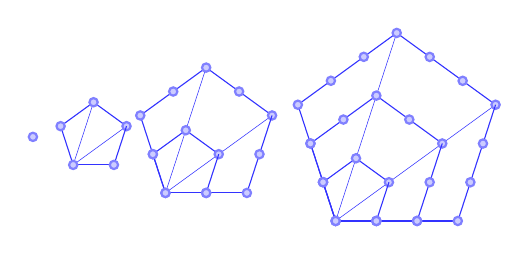
\begin{tikzpicture}
      [scale=.11
      ,ver/.style={circle,draw=blue!50,fill=blue!20,thick,inner sep=0,minimum size=3}
      ,lin/.style={color=blue!80}]
        \coordinate (A0) at (0,0);
        \coordinate (A1) at (7,0);
        \coordinate (A2) at (20,0);
        \coordinate (A3) at (42,0);
        \node[ver] at (A0){};
        \draw[lin,very thin] (A1) + (-126:4) -- +(18:4);
        \draw[lin,very thin] (A1) + (-126:4) -- +(90:4);
        \foreach \a in {18,90,...,306}{
          \draw[lin] (A1)
                                       +(\a:4)    node[ver]{}
                                    -- +(\a+72:4);
        }
        \draw[lin,very thin] (A2) + (-126:8) -- +(18:8);
        \draw[lin,very thin] (A2) + (-126:8) -- +(90:8);
        \foreach \a in {18,90,...,306}{
          \draw[lin] (A2)
                                       +(\a:8)    node[ver]{} coordinate (A)
                                    -- +(\a+72:8)             coordinate (B);
          \node[ver] at  ($ (A)!.5!(B) $){};
          \draw[lin] (A2) ++ (-126:8) ++ (54:4)
                                       +(\a:4)    node[ver]{} coordinate (A)
                                    -- +(\a+72:4)             coordinate (B);
        }
        \draw[lin,very thin] (A3) + (-126:12) -- +(18:12);
        \draw[lin,very thin] (A3) + (-126:12) -- +(90:12);
        \foreach \a in {18,90,...,306}{
          \draw[lin] (A3)
                                       +(\a:12)    node[ver]{} coordinate (A)
                                    -- +(\a+72:12)             coordinate (B);
          \node[ver] at  ($ (A)!.333!(B) $){};
          \node[ver] at  ($ (A)!.666!(B) $){};
          \draw[lin] (A3) ++ (-126:12) ++ (54:8)
                                       +(\a:8)    node[ver]{} coordinate (A)
                                    -- +(\a+72:8)             coordinate (B);
          \node[ver] at  ($ (A)!.5!(B) $){};
          \draw[lin] (A3) ++ (-126:12) ++ (54:4)
                                       +(\a:4)    node[ver]{} coordinate (A)
                                    -- +(\a+72:4)             coordinate (B);
        }
      \end{tikzpicture}
}{7cm}{\risn Пятиугольные числа.}
\vspace{-4mm}
\УстановитьГраницы{0truecm}{6.5truecm}



% \задача
% Сформулируйте и докажите теорему, описывающую явление: \\
% $3+5=2^3$,~$7+9+11=3^3$,~$13+15+17+19=4^3$,~$\ldots$
% \кзадача

\задача
{\it Пятиугольные числа} $P_1=1$, $P_2=5$,
$P_3=12$, $P_4=22$, $\ldots$  показаны на рисунке~2.
Найдите разность $P_k-P_{k-1}$
между последовательными пятиугольными числами.
Выразите $P_n$ через~$n$.
\кзадача

\задача Докажите геометрически, что сумма $n$-го треугольного и $n$-го
четырёхугольного числа на $n$ больше, чем $n$-ое пятиугольное число, .
\кзадача
\ВосстановитьГраницы
